\section{Forma recursiva}
\markright{FORMA RECURSIVA}

Ahora se verá como crear cualquier búsqueda exhaustiva con recursión, lo cual nos va a servir para cualquier fuerza bruta que no hayamos visto en la lista anterior. Es la forma general de cualquier exhaustiva.

Para resolver esto, imaginaremos que lo que queremos buscar es una una secuencia de valores que cumplan algo. 

Si nos fijamos, todos los ejemplos anteriores fueron eso, buscar una secuencia de valores:

Por ejemplo, en la búsqueda lineal buscábamos una secuencia de un solo número, por ejemplo \([4]\) que representa el valor de la raíz cuadrada de \(16\). Mientras que en las parejas de elementos queríamos una secuencia de dos números que representen la pareja, por ejemplo \([1, 6]\), los indices de un arreglo.

En los ordenes, la permutación tal cual es la secuencia, y en los subconjuntos teníamos una cadena de tamaño n con valores de 0 o 1 representando si un elemento esta o no.

Ahora, la pregunta es ¿cómo buscamos las secuencias de números? para una secuencia lo que podemos imaginar es que tomamos la decisión de cuanto vale el primer elemento de la secuencia, luego elegimos cuanto vale el segundo elemento, luego el tercero, etc. Formando una cadena de decisiones hasta que lleguemos al final de la secuencia.

\begin{center}
	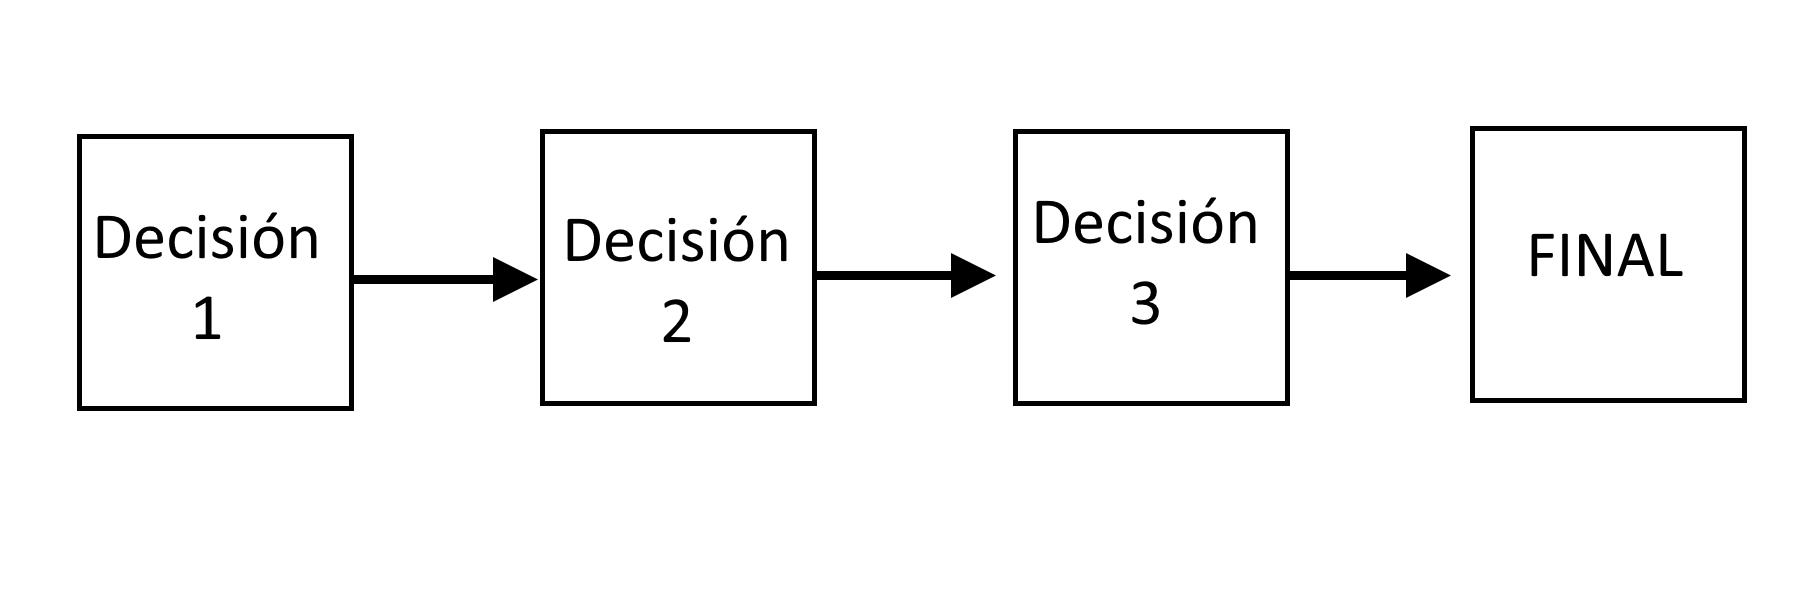
\includegraphics[scale=0.2]{decisiones}
\end{center}

Y la idea de esta búsqueda completa es revisar todas las formas posibles de tomar esta serie de decisiones para encontrar todas las cadenas. 

Para esto hacer esto, cada que tengamos que tomar una decisión, probamos todas las opciones disponibles para ver que producen.

Supongamos que estamos buscando la solución y tenemos una decisión ante nosotros con dos opciones. Lo que la búsqueda exhaustiva hace es ver ``¿qué pasa si elijo la primera opción?" para luego revisar ``¿Y qué sucede con la segunda opción?". Si después hay más decisiones, también explorara todas las opciones que aporten.

De forma que la búsqueda se ve aproximadamente de la siguiente forma:

\begin{lstlisting}
	busqueda(decision, solucion) {
		if (decision es el final) {
			revisar solucion contruida;
			return;
		}		
		//Revisa cada opcion de esta decision:
		for (int i=0; i < decision.opciones; i++) {
			busqueda(siguiente_decision, solucion+ decision.opcion[i] );
		}
	}
\end{lstlisting}

Probablemente reconozcas este código de la forma recursiva de iterar por todos los subconjuntos, esto es porque utilizamos esta técnica para resolver aquella fuerza bruta.

Como es costumbre, veamos ejemplos para entender esto:
\subsection*{Ejemplo: Pares de suma K}
Dado un arreglo \(A\) de \(N\) enteros, determina si existe un par \(i\) y \(j\) (\(i<j\)) tal que \(A[i]+A[j]==K\).

\subsection*{Ejemplo}
\begin{casebox2}
	\scase{
		5 8\\
		3 1 2 5 9
	} 
	{SI}
	\scase{
		5 10\\
		3 4 2 12 9
	} {
		NO
	}
	
\end{casebox2}
\subsubsection*{Límites}
\begin{plimits}
	\item \(1\leq N \leq 10^3\)
	\item \(1\leq A[i], K \leq 10^9\)
\end{plimits}

\subsection*{Solución}
Este problema lo vimos en la sección de iterar por pares,lo que debíamos hacer era revisar todas las posibles parejas y ver si existía aquella que sume \(K\).

\begin{lstlisting}
	bool respuesta=false;
	for (int i=0; i < N;i++) {
		for (int j=i+1; j < N; j++) {
			if (A[i]+A[j]==K) {
				respuesta=true;
			}
		}
	}
\end{lstlisting}

Pero ahora pensemos un poco a más profundidad que hace este código.

Primero va revisando todas las opciones de \(i\). Y para cada opción, evalúa todas las opciones para \(j\). 

Tiene que elegir cuanto valen dos valores, probará todos los valores para \(i\) con el primer ciclo, revisando un valor por cada iteración. Y para cada valor de \(i\) probará todos los valores de \(j\) posibles.

Esto se puede ver también con una recursión:
\pagebreak

\begin{lstlisting}
int solucion[3];
bool respuesta=false;
void buscar(int decision) {
	if (decision==3) {
		//Ya tomamos las dos decisiones, cuanto vale i, cuanto vale j. Revisemos esta solucion
		if (A[solucion[1]]+A[solucion[2]]==K) {
			respuesta=true;
		}
		return;
	}
	if (decision == 1) {
		//toca decidir cuanto vale i. Como esto es busqueda completa, revisaremos cada opcion.
		for (int i=0;i < N; i++) {
			solucion[decision]=i;//agregar i a la solucion
			buscar(decision+1);	
			solucion[decision]=-1;//quitar i de la solucion
		}
	} else {
		//toca decidir cuanto valdra j. Probemos todos los valores
		for (int j= solucion[1]+1; j< N;j++) {				
			solucion[decision]=i;//agregar j a la solucion
			buscar(decision+1);
			solucion[decision]=i;//quitar j.
		}
	}
}


int main() {
	[...]
	buscar(1);
	cout << "NO";
	return 0;
}
\end{lstlisting}

Estos dos códigos siguen la misma idea de obtener los pares fijando primero un valor de \(i\), y  luego fijando un valor para \(j\); solo lo realizan de una forma diferente.

\textbf{Consejo:} Entiende porque los dos códigos resuelven el problema con la misma idea antes de continuar, prueba a ejecutar ambos a mano con lápiz y papel.

Básicamente el primer código hace lo siguiente para explorar todos los pares:
\begin{center}
	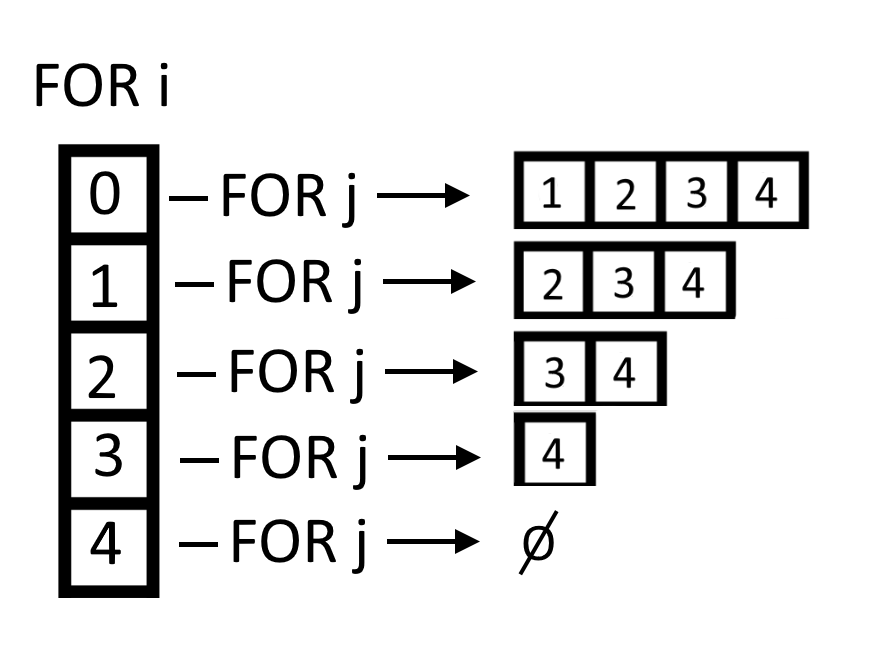
\includegraphics[scale=0.3]{forbrute}
\end{center}

Donde para cada elemento de la lista de valores de \(i\), prueba los valores de \(j\).

Mientras que el segundo hace recursión para obtener todos los pares posibles.

\begin{center}
	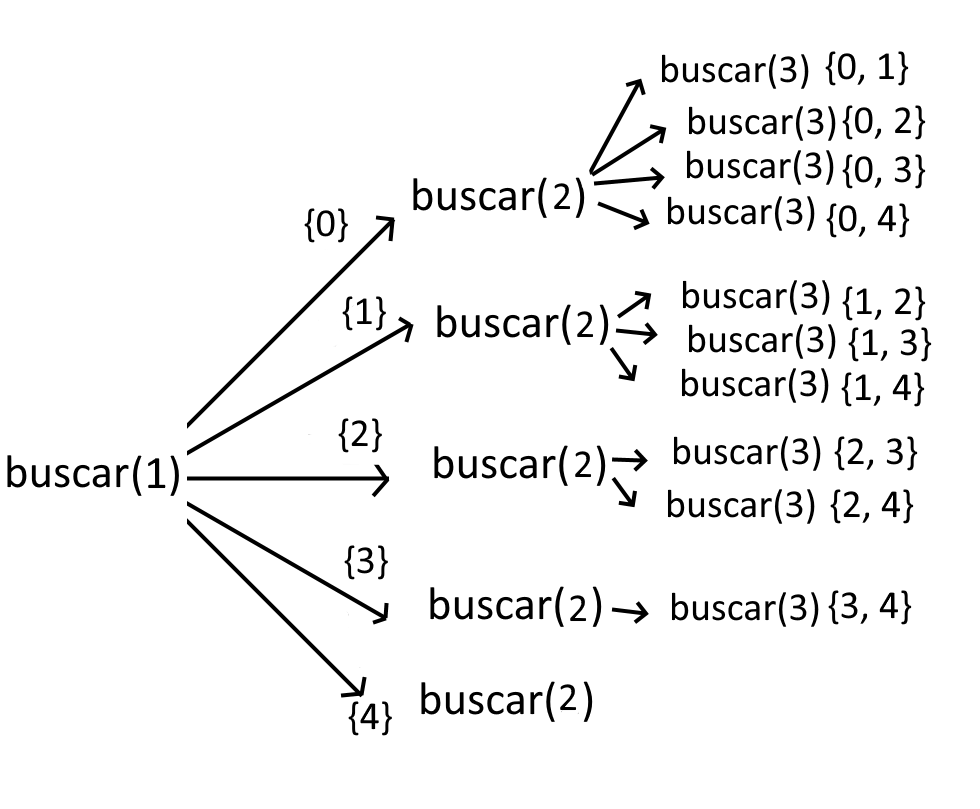
\includegraphics[scale=0.3]{paresrec}
\end{center}

Ambos son búsquedas exhaustivas que exploran todas las formas de tomar las decisiones de elegir \(i\) y luego \(j\).

Veamos otro ejemplo:

\subsection*{Ejemplo: Dividir en tres grupos}
Una clase se ha juntado para jugar LaserTag. Por el diseño del lugar donde van a jugar han decidido formar tres equipos, pero quieren que los jugadores sean repartidos justamente.

La clase consiste de \(n\) estudiantes. El estudiante \(i\) tiene \(a_i\) habilidad para el LaserTag. 

Los equipos están repartidos de forma justa si la suma de la habilidad de sus integrantes es igual para los tres equipos y nadie se queda sin equipo.

Determina si se puede formar los equipos de forma justa y si sí, determina la repartición.

\textbf{Entrada}\\
Un entero \(n\), indicando la cantidad de estudiantes en la clase.

La segunda línea tendrá \(n\) enteros \(a_1, a_2, \ldots, a_n\), donde \(a_i\) es la habilidad del estudiante \(i\).

\textbf{Salida}\\
Si no se puede hacer la repartición imprime \verb|NO|.

En caso de que se pueda, en la primera línea imprime \verb|SI|.

En la segunda línea imprime \(n\) enteros. El \(i\)-ésimo entero sera 1, 2 o 3 dependiendo de a que equipo va el estudiante \(i\). 

Si hay varias soluciones, se acepta cualquiera.

\begin{samepage}
	\textbf{Ejemplo}\\
	\begin{casebox3}
		\ecase{
			6\\
			3 1 6 2 4 2  
		}{
			SI\\
			1 1 3 2 2 1
		}{
			El primer equipo tiene una habilidad\\ de
			\(3+1+2\).
			\\
			\\
			El segundo tiene habilidad de \(2+4\).
			\\
			\\
			Y el tercer equipo tiene un\\ integrante de \(6\).
		}
		\ecase{
			6\\
			2 1 5 2 3 4
		}{NO}{No se puede repartir a\\ los estudiantes justamente.}
	\end{casebox3}

\end{samepage}

\textbf{Límites}
\begin{plimits}
	\item \(1\leq N \leq 15\)
	\item \(1\leq a_i \leq 10^6\)
\end{plimits}

ENLACE: TODO

\subsection*{Solución}

Como siempre, antes de leer la solución te invitamos a que trates de resolver el problema por un rato.

Entonces, podemos pensarlo como que tenemos \(N\) decisiones, donde cada decisión es ¿A que equipo envío al estudiante \(i\)?

Y lo podemos imaginar como que los estudiantes se forman delante de nosotros y les vamos diciendo: "Equipo 1, equipo 2, equipo 1, equipo 3, ... ".

Entonces, podemos hacer un código que haga eso, que vaya tomando las decisiones de enviar a cada estudiante al equipo 1, 2 o 3.

Para esto crearemos la función repartir(int c, int equipo1, int equipo2, int equipo3) que se encargara de decidir a cual equipo mandar al estudiante \(c\). 
Y llevaremos cuenta de cuanta habilidad lleva cada equipo hasta ahora.

Además usaremos un arreglo \verb|reparticion[]| para llevar cuenta de a que equipo mandamos cada estudiante.

\pagebreak

\begin{lstlisting}
	int n;
	int a[16];
	int reparticion[16];
	void repartir(int c, int equipo1, int equipo2, int equipo3) 
	{
		//Mandar el estudiante c al equipo1:
		reparticion[c]=1;
		repartir(c+1, equipo1+a[c], equipo2, equipo3);
		
		//Mandar el estudiante c al equipo2:
		reparticion[c]=2;
		repartir(c+1, equipo1, equipo2+a[c], equipo3);
		
		//Mandar el estudiante c al equipo2:
		reparticion[c]=3;
		repartir(c+1, equipo1, equipo2, equipo3+a[c]);
	}
\end{lstlisting}

Ahora, le falta la condición de paro. Esto será en el momento que ya no tengamos estudiantes que repartir, cuando \(c=n\).

Además, aprovecharemos allí para validar que la repartición sea justa. Si lo es, imprimiremos esta construcción como respuesta y terminaremos el programa.
\pagebreak
\begin{lstlisting}
	int n;
	int a[16];
	int reparticion[16];
	void repartir(int c, int equipo1, int equipo2, int equipo3) 
	{
		if (c==n) {
			if (equipo1==equipo2 && equipo1==equipo3) {
				cout << "SI\n";
				for (int i =0;i<n; i++) 
				cout << reparticion[i]<<" ";					
				exit(0);
			}
			return;
		}
		//Mandar el estudiante c al equipo1:
		reparticion[c]=1;
		repartir(c+1, equipo1+a[c], equipo2, equipo3);
		
		//Mandar el estudiante c al equipo2:
		reparticion[c]=2;
		repartir(c+1, equipo1, equipo2+a[c], equipo3);
		
		//Mandar el estudiante c al equipo2:
		reparticion[c]=3;
		repartir(c+1, equipo1, equipo2, equipo3+a[c]);
	}
	int main() {
		ios_base::sync_with_stdio(0); cin.tie(0);
		cin >> n;
		for (int i =0; i< n; i++) {
			cin >> a[i];
		}
		repartir(0, 0, 0, 0);
		cout << "NO";
	}
	
\end{lstlisting}

\subsection{Complejidad}

La complejidad de una búsqueda exhaustiva varia mucho dependiendo de que tipo de solución se esta buscando, en el primer ejemplo terminamos con una complejidad de \(O(N^2)\). 

Pero la complejidad del ejemplo anterior es \(O(3^N)\). Esto es porque la complejidad de la búsqueda exhaustiva es \(O(candidatos)\) y en este caso, las formas de repartir se multiplican por tres por cada estudiante que se agregue a la clase, ya que tenemos todas las opciones de equipos anteriores, pero unas con el nuevo en el 1, otros con el equipo 2, y otra vez con el estudiante en el 3.


\section*{Problemas de práctica}
\addcontentsline{toc}{section}{Problemas de práctica}
\begin{exercise}
	\problema{Encontrar posición en un arreglo}{TODO}

	NOTA: Utiliza recursión.
\end{exercise}

\begin{exercise}
	\problema{Contando LaserTag justos}{TODO}
\end{exercise}
\begin{exercise}
	\problema[torre-I]{Subiendo la torre}{TODO}
\end{exercise}

\begin{exercise}
	\problema{Mapas}{\omegauplink{OMI-2020-Mapas}}
\end{exercise}


